\subsection{Synthesis of Research Gaps}

A systematic review of the collected literature in sensor-based anomaly detection, quantum computing for optimization, and agentic AI systems reveals that while each individual domain has achieved substantial progress independently, the integration of these three paradigms within a single, empirically grounded, closed-loop framework for smart manufacturing predictive maintenance remains absent. This chapter derives five research gaps from the convergent evidence of the literature, grounds each gap in the concrete statistical properties of the 100,000-reading smart manufacturing dataset, and formalizes the research problem that QASAMAP addresses.

\subsection{Gap 1: Siloed Treatment of Anomaly Detection, Prognostics, and Scheduling}

The most pervasive gap in the existing literature is the treatment of anomaly detection, remaining useful life estimation, and maintenance scheduling as three entirely separate problems. Comprehensive surveys of deep learning anomaly detection --- including Chalapathy and Chawla (2019) \cite{Chalapathy2019} and Pang et al.\ (2021) \cite{pang_deep_2021} --- cover hundreds of papers without identifying a single work that jointly optimizes anomaly detection, RUL prediction, and maintenance scheduling within a unified pipeline. Multi-sensor anomaly detection works \cite{zhang_unsupervised_2021, Gao2022} demonstrate superior sensor fusion but treat anomaly detection as a terminal task rather than the first stage of a full predictive maintenance workflow.

The empirical consequences of this siloed treatment are directly observable in the research dataset. The anomaly flag, predicted RUL, failure type, and maintenance required label are all statistically interdependent: temperature correlates with anomaly flag at $r = 0.447$, anomaly flag correlates with downtime risk at $r \approx 1.0$, and RUL correlates with downtime risk at $r = -0.436$. The 16,333 readings with RUL below 50 hours represent machines that are simultaneously anomalous and prognostically critical --- a dual characterization that joint modeling can exploit far more effectively than two independent models. QASAMAP addresses this gap by integrating T-GCN-based forecasting, tree-based classification, and quantum-agentic decision orchestration within a single closed-loop architecture.

\subsection{Gap 2: Classical Intractability of Fleet-Level Maintenance Scheduling}

The second research gap concerns the scalability of maintenance scheduling optimization across large machine pools. Machine maintenance scheduling belongs to the NP-hard combinatorial optimization class, for which quantum algorithms offer provable computational advantages at sufficient problem scales \cite{Blekos2024}. The 19.70\% maintenance rate observed in the research dataset implies that approximately 10 machines in a 50-machine pool require concurrent maintenance attention at any time, and determining globally optimal intervention sequences requires evaluating a combinatorially large solution space that classical greedy and genetic algorithm approaches can only partially navigate \cite{symons_practitioners_2023}.

The QASAMAP implementation directly addresses this gap through the \texttt{QuantumAnnealingOptimizer} and \texttt{QAOAScheduler} classes in \texttt{quantum\_agent.py}. The QUBO formulation minimizes $-\sum_i(w_i \cdot x_i) + \lambda(\sum_i x_i - k)^2$, where $w_i$ is the quantum risk score of machine $i$, $x_i \in \{0,1\}$ is the binary maintenance assignment variable, and $\lambda$ enforces a cardinality constraint on the number of machines selected for immediate attention. The QAOA scheduler then partitions all machines into immediate (Slot~A) and planned (Slot~B) maintenance windows by maximizing a MaxCut objective on the machine conflict graph, augmented with Pauli-Z bias terms that steer high-risk machines toward Slot~A.

\subsection{Gap 3: Static Model Architectures in Non-Stationary Environments}

The third gap concerns the universal adoption of static, train-then-deploy architectures that cannot adapt to distributional shifts inherent in real industrial operations. Works such as Zeng et al.\ (2024) \cite{lee_autoencoder-based_2024} develop sophisticated static detectors with no adaptation mechanism, and the temporal analysis of the research dataset confirms the need for adaptability: daily anomaly rates fluctuate significantly around the 8.92\% mean, reflecting non-stationary operating conditions. Without autonomous model adaptation, deployed systems degrade in accuracy over time as sensor distributions evolve.

QASAMAP addresses this gap through the \texttt{LearningLoop} class in \texttt{quantum\_agent.py}, which evaluates false positive and false negative rates from the \texttt{feedback\_log} after each decision cycle. When false positive rates exceed 40\%, warning thresholds for temperature and vibration are automatically relaxed; when false negative rates exceed 20\%, warning thresholds are tightened. A quantum feedback mechanism cross-checks Pauli-Z anomaly labels against final agent actions to identify potential quantum false negatives (Q-FN) --- cases where the quantum circuit detected sensor danger below the classical threshold but the agent issued only a passive monitoring action. When sufficient feedback accumulates (minimum 5 records), a retraining payload is exported to trigger T-GCN model updates.

\subsection{Gap 4: Absence of Quantum-Enhanced Risk Encoding for Industrial Sensors}

The fourth gap is the limited application of quantum feature encoding to industrial sensor risk assessment. The quantum machine learning literature has demonstrated quantum kernel advantages for minority class classification \cite{kreplin_squlearn_2025}, but applications to multi-sensor industrial risk encoding are rare. The research dataset presents the conditions under which quantum encoding advantages are most theoretically expected: five correlated sensors, severe failure class imbalance (Electrical Fault: 1,014 instances vs.\ Normal: 91,899), and complex nonlinear risk relationships between sensors that share similar anomaly rates (8.80--9.86\% across failure types) but distinct per-sensor signatures.

The \texttt{PauliZRiskEncoder} class in QASAMAP addresses this gap. For each machine, normalized sensor values are encoded as RZ rotation angles $\theta_i = \pi \cdot \text{norm}_i$, Hadamard gates create superposition, and CNOT gates between adjacent sensor qubits capture inter-sensor correlations. The per-sensor Pauli-Z expectation is $\langle Z_i \rangle = \cos(\pi \cdot \text{norm}_i)$, mapping sensors from the safe regime ($\langle Z \rangle \to +1$) through marginal ($\langle Z \rangle \to 0$) to the danger regime ($\langle Z \rangle \to -1$). A weighted composite $\langle Z \rangle_c = \sum_i w_i \langle Z_i \rangle$ (weights: temperature 0.30, vibration 0.30, humidity 0.15, pressure 0.15, energy 0.10) produces a machine-level quantum risk label that drives the quantum override mechanism.

\subsection{Gap 5: Absence of Integrated Agentic Orchestration for Maintenance Decision Support}

The fifth gap is the absence of agentic AI frameworks that simultaneously achieve autonomous maintenance decision orchestration, quantum integration, interpretability, and continuous learning within a single industrial system. Works on LLM-based sensor reasoning (LLMSense \cite{ouyang_llmsense_2024}, DeepSQA \cite{xing_deepsqa_2021}) demonstrate natural language interfaces for sensor data but do not integrate quantum signals, closed-loop feedback, or multi-agent action coordination. QASAMAP closes this gap through the \texttt{MultiAgentOrchestrator} class, which sequences four LLM agents (Monitoring, Diagnosis, Planning, Reporting) such that each agent's output feeds the next, quantum override signals are injected at the orchestration level, and all decisions are logged for feedback-based learning.

\subsection{Formal Problem Formulation}

The QASAMAP research problem is to jointly learn and deploy five functional components:

\begin{enumerate}
    \item A T-GCN spatiotemporal forecasting function $\Psi_{\text{T-GCN}}: \mathbb{R}^{W \times 7 \times N} \to \mathbb{R}^{H \times 5 \times N}$ that maps windowed multivariate sensor sequences across $N$ machines to $H$-step ahead forecasts, exploiting the cross-correlation lag graph $G = (V, E, W)$ constructed over the machine pool.

    \item A supervised classification and regression function $\Phi: \mathbb{R}^{d} \to (Y_c^{(1)} \times \cdots \times Y_c^{(5)} \times \mathbb{R}_+)$ that maps a sensor feature vector to five classification outputs (machine status, anomaly flag, failure type, downtime risk, maintenance required) and one regression output (predicted RUL), using tree-based ensemble or deep tabular models.

    \item A quantum risk encoding function $\Gamma: \mathbb{R}^{5} \to [-1, +1]$ implemented via Pauli-Z multi-sensor encoding that maps a machine's five normalized sensor values to a composite quantum expectation value $\langle Z \rangle_c \in [-1, +1]$ and a quantum risk label $\ell \in \{\texttt{QUANTUM-ANOMALY}, \texttt{QUANTUM-WARN}, \texttt{QUANTUM-MARGINAL}, \texttt{QUANTUM-NORMAL}\}$.

    \item A QUBO priority ranking and QAOA scheduling function $\Omega: \{q_i\}_{i \in M} \to (\text{ranking}, \{0,1\}^{|M|})$ that maps machine quantum risk scores to an ordered machine priority ranking (via QUBO annealing) and a binary slot assignment vector (via QAOA) partitioning all machines into immediate and planned maintenance windows.

    \item A multi-agent agentic system $\mathcal{A} = \{\text{Mon}, \text{Diag}, \text{Plan}, \text{Rep}\}$ that autonomously orchestrates the execution of $\Psi_{\text{T-GCN}}$, $\Phi$, $\Gamma$, and $\Omega$ in a closed-loop architecture with contextual memory, quantum override logic, and continuous threshold adaptation.
\end{enumerate}

\subsection{Proposed Methodology --- QASAMAP Framework}

\subsubsection{Framework Overview}

The QASAMAP framework is structured as a seven-layer closed-loop pipeline in which raw sensor data flows upward through data ingestion, T-GCN forecasting, supervised prediction, quantum encoding, quantum optimization, agentic orchestration, and learning loop layers, while feedback and threshold update signals flow downward to continuously refine lower-layer parameters. This bidirectional architecture directly addresses Gap~3 by enabling autonomous adaptation without manual retraining cycles.

Figure~\ref{fig:research_methodology} illustrates the overall three-layer architecture at a high level, while Figures~\ref{fig:tgcn_architecture}, \ref{fig:agentic_ai_architecture}, and \ref{fig:quantum_agent_architecture} provide detailed views of the T-GCN pipeline, the Agentic AI orchestration system, and the integrated Quantum-Agentic decision loop respectively.

\subsubsection{Layer 1: Sensor Data Acquisition and Stream Management}

The data acquisition layer ingests continuous sensor streams from 50 machines, each producing five sensor readings (temperature, vibration, humidity, pressure, energy consumption) at one-minute intervals. The \texttt{kafka\_consumer\_simulation} function in both \texttt{agenticai.py} and \texttt{quantum\_agent.py} implements a Kafka consumer abstraction that delivers sensor events as normalized dictionaries containing machine identifier, timestamp, five sensor values, machine status, anomaly flag, predicted RUL, failure type, downtime risk, and maintenance required. In production deployment, this simulation is replaced by a live \texttt{KafkaConsumer} connecting to the factory's \texttt{sensor\_stream} topic.

The \texttt{normalize\_event} function standardizes incoming events into a canonical dictionary format, resolving field name variations and applying default values for missing fields. The \texttt{group\_events\_by\_machine} function organizes the stream into per-machine event lists, enabling the quantum layer to process one representative event per machine before initiating the per-machine agentic pipeline. Sensor quality bounds derived from the dataset's physical ranges (temperature: 35.55--121.94\textdegree C; vibration: $-$17.09 to 113.80; humidity: 30.00--80.00\%; pressure: 1.00--5.00 bar; energy: 0.50--5.00 kWh) are stored in the \texttt{SENSOR\_BOUNDS} dictionary for downstream Pauli-Z normalization.

\subsubsection{Layer 2: T-GCN Spatiotemporal Forecasting}

The T-GCN layer provides 30-minute ahead forecasts of all five sensor channels across the 50-machine pool, implemented in \texttt{tcgn\_updated.py} and structured around four stages.

\begin{figure}[htbp]
    \centering
    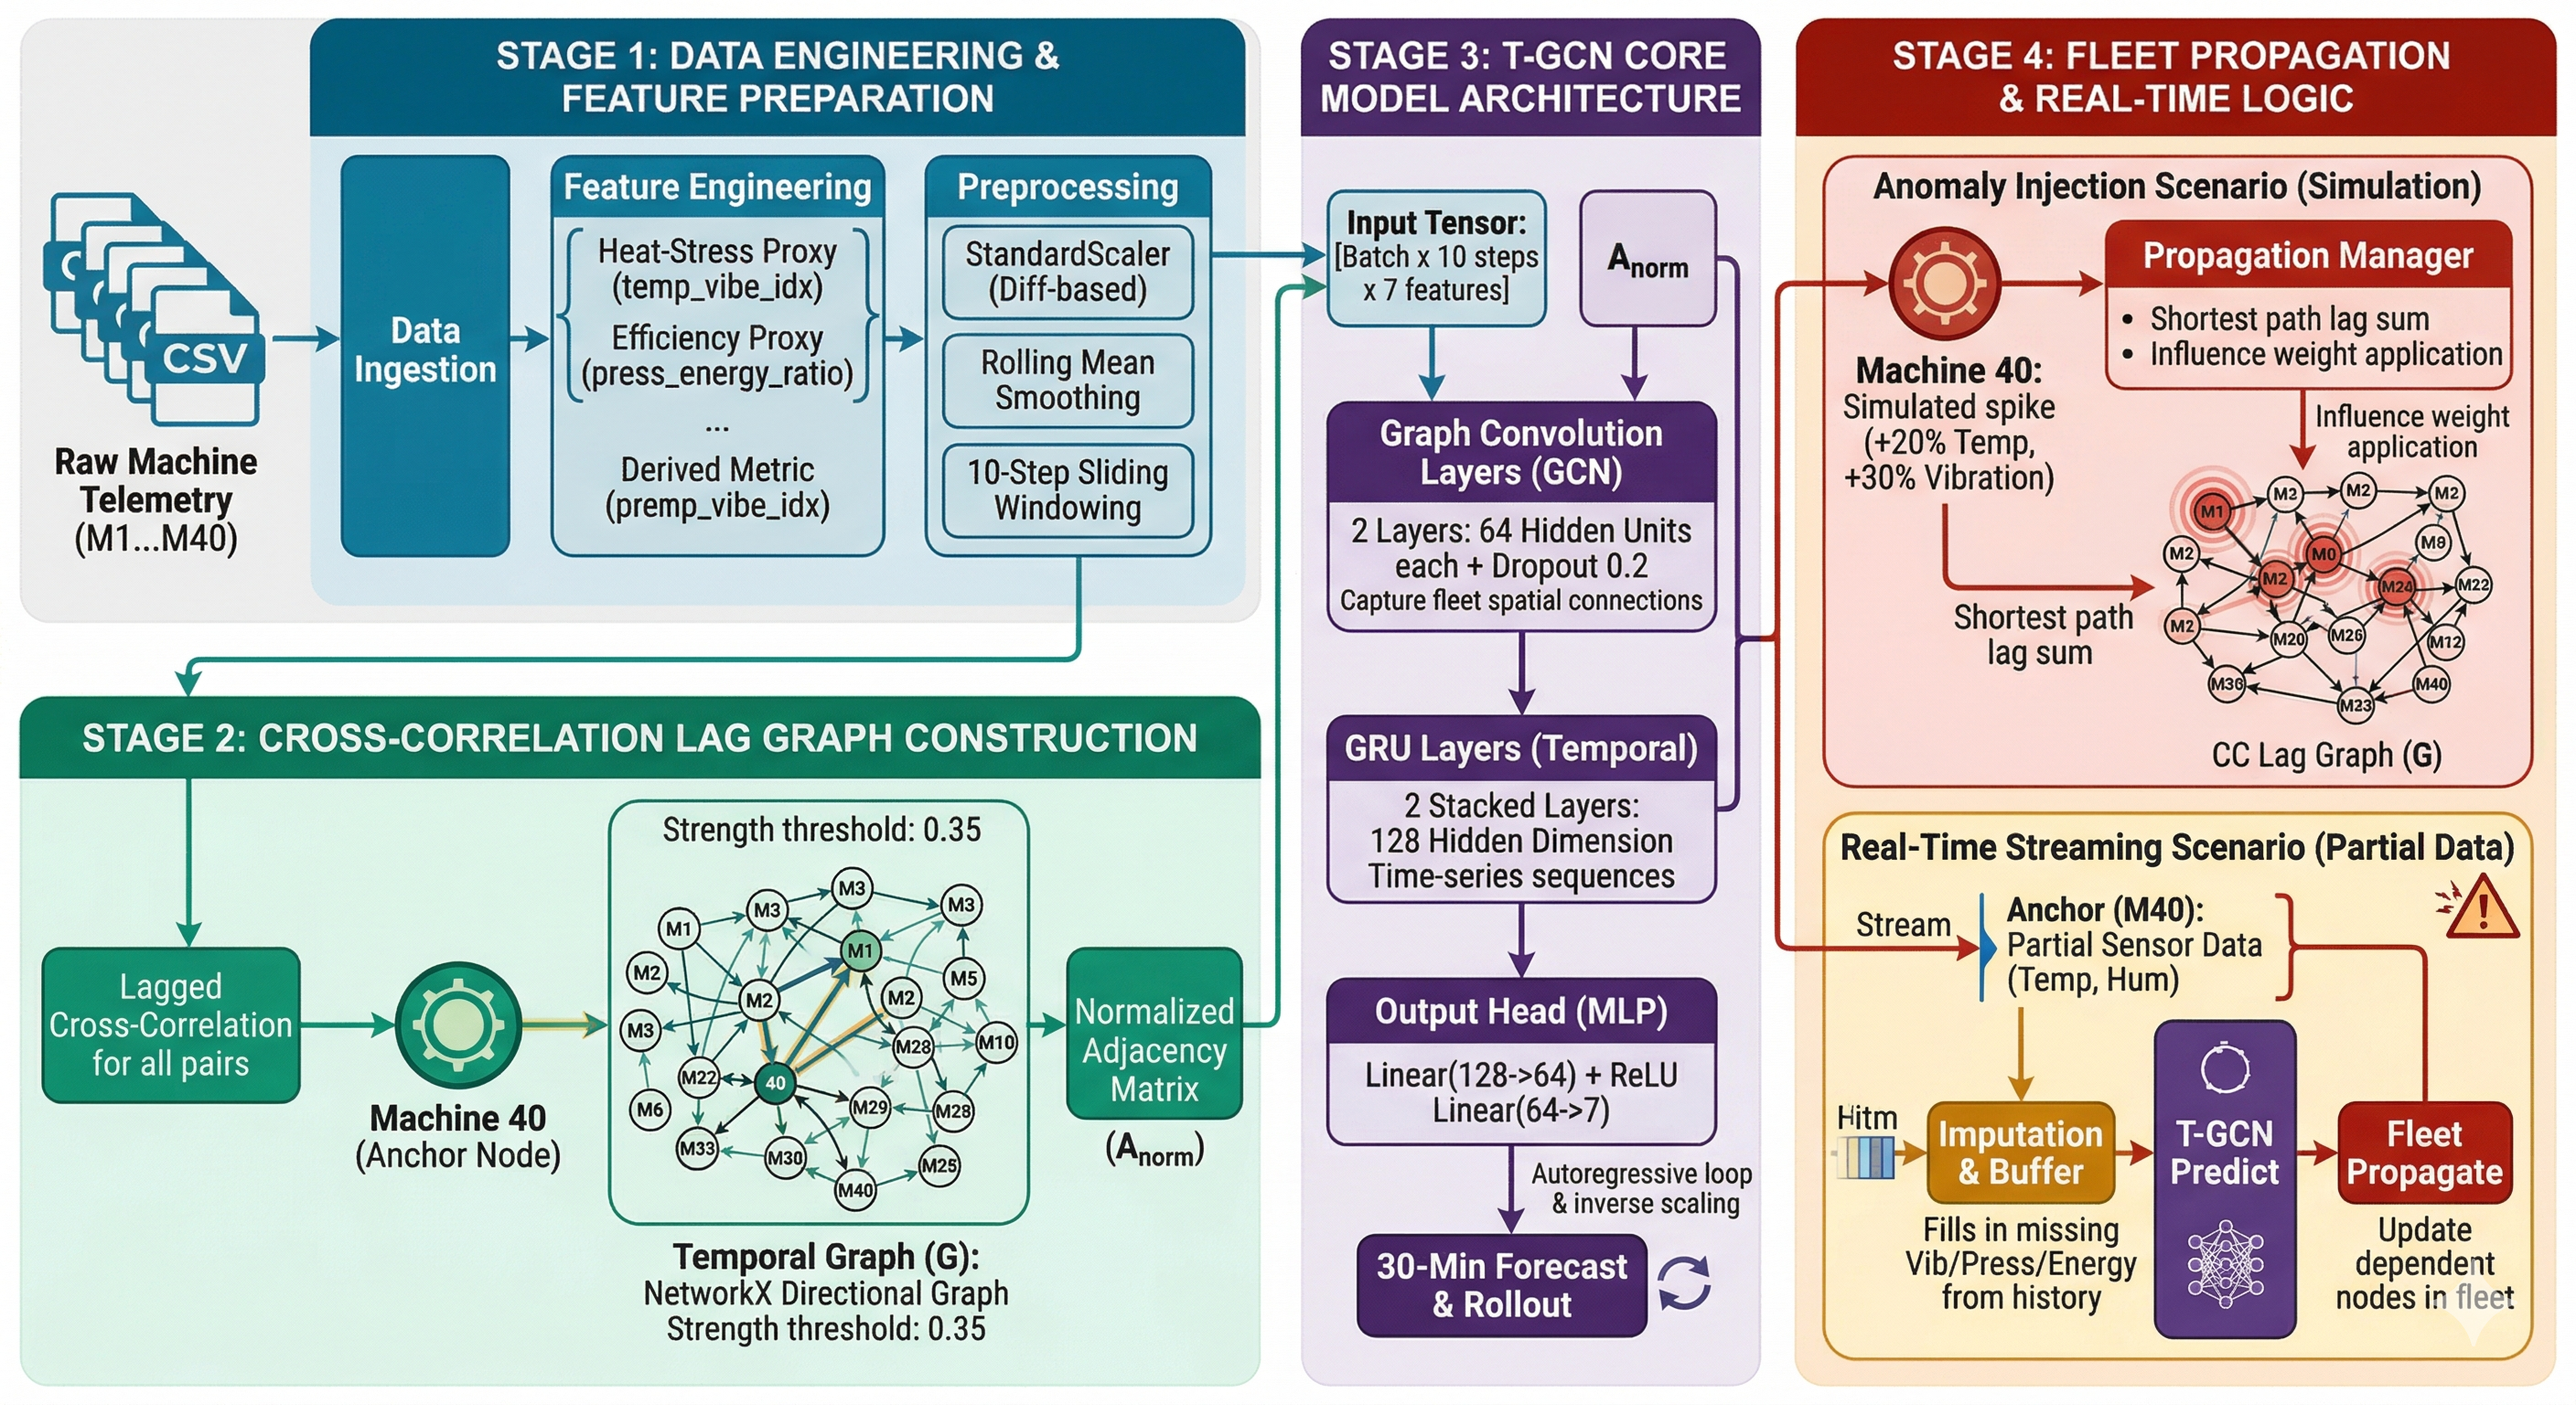
\includegraphics[width=\textwidth]{figures/tgcn_architecture.png}
    \caption{T-GCN four-stage pipeline: Stage~1 (data engineering and feature preparation with \texttt{temp\_vibe\_idx} and \texttt{press\_energy\_ratio}), Stage~2 (cross-correlation lag graph construction with 50 nodes, 538 edges, and Machine~40 as anchor node), Stage~3 (T-GCN core with Graph Convolution and GRU layers), and Stage~4 (machine-wide propagation with anomaly injection and real-time streaming via \texttt{AnchorBufferManager}).}
    \label{fig:tgcn_architecture}
\end{figure}

\paragraph{Stage 1: Data Engineering and Feature Preparation.} Raw sensor readings are augmented with two engineered features: a heat-stress proxy \texttt{temp\_vibe\_idx} = temperature $\times$ vibration, capturing combined thermal and mechanical loading; and an efficiency proxy \texttt{press\_energy\_ratio} = energy\_consumption / (pressure + 0.1), capturing hydraulic efficiency degradation. The resulting seven-variable feature set is preprocessed using sensor-specific rolling mean smoothing (window~10 for vibration, 5 for others), first-order differencing for stationarity, and StandardScaler normalization fitted on the training split. A 10-step sliding window partitions the differenced, scaled sequences into input-output training pairs.

\paragraph{Stage 2: Cross-Correlation Lag Graph Construction.} The T-GCN spatial structure is defined by a directed graph $G = (V, E, W)$ constructed from pairwise lagged cross-correlations of the temperature time series. For each machine pair $(m_i, m_j)$, the \texttt{compute\_machine\_lag\_matrix} function computes the Pearson correlation at integer lags from $-10$ to $+10$ timesteps, recording the lag and strength at maximum absolute correlation. Edges are added when the correlation strength exceeds 0.35, yielding 50 nodes and 538 directed edges. The normalized adjacency matrix is $A_{\text{norm}} = D^{-1/2} A D^{-1/2}$, where $D$ is the degree matrix. Machine~40 is designated as the anchor node based on its highest out-degree centrality among all machines.

\paragraph{Stage 3: T-GCN Core Model.} The \texttt{TemporalGCN} class implements two Graph Convolution layers (64 hidden units, Dropout 0.2) for spatial information propagation across the machine graph at each timestep, followed by two stacked GRU layers (128 hidden units, Dropout 0.2) for temporal evolution modeling. The output head is a two-layer MLP (Linear(128$\to$64) + ReLU + Linear(64$\to$7)) that predicts next-step differenced sensor values, which are inverse-transformed to original-scale forecasts. Training uses the Adam optimizer (lr = 0.0005, weight decay = 1e-5) with cosine annealing and gradient clipping at norm 1.0 for 15 epochs.

\paragraph{Stage 4: Machine-Wide Propagation and Streaming.} The \texttt{propagate\_from\_anchor} function implements baseline and anomaly injection machine-wide propagation. In the anomaly scenario, Machine~40's input window receives a $+$20\% temperature and $+$30\% vibration spike; dependent machines are perturbed by $w \cdot \epsilon$ (propagation weight $w$, perturbation factor $\epsilon = 0.02$) before their own T-GCN rollout. The \texttt{AnchorBufferManager} handles partial sensor streams from Machine~40 (temperature and humidity only), imputing missing values from the T-GCN's previous prediction and maintaining a sliding buffer for continuous streaming inference.

\subsubsection{Layer 3: Supervised Classification and Regression}

The supervised prediction layer evaluates five tree-based ensemble models (XGBoost, LightGBM, CatBoost, HistGradientBoosting) and TabNet for six machine health prediction targets as implemented in \texttt{regression\_classification\_model\_experiment.py}. Five classification targets (machine status, anomaly flag, failure type, downtime risk, maintenance required) are evaluated using Accuracy, Precision, Recall, F1-score, AUC-ROC, and Matthews Correlation Coefficient (MCC). One regression target (predicted RUL) is evaluated using MAE, RMSE, R\textsuperscript{2}, and Explained Variance. Class imbalance in the failure type and maintenance required targets is handled through class-weight balancing in the ensemble learners and focal loss in TabNet.

\subsubsection{Layer 4: Quantum Computing Enhancement (overview)}

The quantum computing layer integrates two NISQ-honest components evaluated on Qiskit Aer statevector simulators: a Pauli-Z entangled compound encoder for sub-threshold multi-sensor anomaly detection, and a QAOA-based scheduler for maintenance time-slot assignment. Both components are pre-registered with explicit hypotheses, statistical tests, and what-can/cannot-be-claimed sections in Chapter~6. Detailed encoding equations, classical baseline comparisons (best single-threshold, multivariate Mahalanobis, weighted-sum classical equivalent of the separable circuit, brute-force enumeration, tuned simulated annealing), and the dedicated reconciliation section addressing the Cerezo et al.\ 2025 quantum-machine-learning skepticism literature are presented in Chapter~6.

\subsubsection{Layer 5: Agentic AI Decision Orchestration (overview)}

The agentic layer implements a multi-agent orchestration system in which specialised LLM-powered agents transform sensor evidence and quantum context into operational maintenance decisions. The agentic architecture is anchored on six pre-registered Value Propositions (zero-shot reasoning, natural-language communication, multi-step pipelines, cross-domain fusion, in-context adaptation, self-reflection) and is empirically evaluated in Chapter~5 through four executed experiments (E1 capability coverage, E3 in-context adaptation, E5 robustness under controlled perturbations, E6 multi-agent vs single-call ablation) and two deferred experiments (E2 cross-domain cold-start with NASA C-MAPSS, E4 operator decision quality user study). Detailed pipeline composition, statistical results, and honest mixed-evidence framing including the E6 counter-result reconciled with the E1 strong result via the breadth-versus-quality distinction are presented in Chapter~5.

\subsubsection{Layer 6: Continuous Learning Loop}

The continuous learning loop evaluates false positive and false negative rates from a persistent feedback log and adjusts classical sensor thresholds adaptively, providing a mechanism by which the deployed system tracks distributional shift in the operating environment without expensive manual retraining cycles. When the feedback log accumulates a sufficient number of records, a structured retraining payload is exported for submission to the T-GCN retraining pipeline, closing the closed-loop adaptation cycle.